\documentclass{article}

\usepackage[ngerman]{babel}

\usepackage[
backend=biber,
style=authoryear,
citestyle=authoryear,
autocite=footnote
]{biblatex}
\addbibresource{bibliography.bib}

\usepackage[toc,page]{packages/appendix}
\usepackage{packages/timeline}

\usepackage{graphicx}
\graphicspath{ {images/} }

\title{Wie entwickelte sich Facebooks Internet.org/Free Basics in Indien?}
\author{
  Fischer, Sarah Susanne\\
  Hein, Oliver\\
  Neidel, Jonathan\\
  Petersen, Tom Magnus\\
  Schmitz, Kai-Ibe\\
  \and
  Als Gruppe `Monopoly' in gemeinsamer Bewertung
}
\date{Dezember 2019}

\begin{document}

\maketitle

\section{Einleitung}

Die folgende Arbeit beschäftigt sich mit der Entwicklung von Facebooks `Internet.org" in Indien. Die Initiative möchte das Internet zu den Menschen bringen, denen das Internet sonst unzugänglich bleiben würde.

\medskip

Indien hat, als eins der bevölkerungsreichsten Länder der Erde mit einer Gesellschaft, die langsam an das Internet angeschlossen wird, enormes wirtschaftliches Potential,
wovon Facebook, mit seinen schwächelnden Nutzerwachstumsumszahlen, gern profitieren möchte.
Um neue Nutzer für die Platform zu gewinnen, soll die Internet.org Initiative genutzt werden, um das Internet zu den bisher unangebundenen Menschen zu bringen.
In seinem ambitionierten Konzept spricht Mark Zuckerberg davon, Menschen durch die Anbindung an globale Märkte, das Wissen der Welt und den Rest der Menschheit aus der Armut zu entheben.

\medskip

Wir möchten der Umsetzung von Internet.org auf den auf den Grunde gehen, um zu erfahren, ob Zuckerberg die Umsetzung seines Versprechens geglückt ist.

Im Zuge dessen beleuchten wir zunächst die Ausgangssitionation: von den Gegebenheiten Indiens (Facebooks Bedeutung in der Bevölkerung, der Umgang mit dem Internet generell, vorherige Begegnungen mit der Netzneutralitätsthematik) zu einer Ausführung von Facebooks Konzept für Internet.org.

Nach Verständnis der Ausgangslage werden die verschiedenen Zeitabschnitte, von der Einführung bis zum Verbot, die Reaktionen der Bevölkerung, sowie die Erfüllung des umschriebenen Nutzens betrachtet.

\break
\tableofcontents
\break

% 1
\section{Ausgangsbedingungen}

Zunächst wird ein Überblick über die Ausgangsbedingungen in Indien geschaffen. Von der Internetverbreitung, ihrer Beziehung zu Facebook, vorherigen Diskussionen zur Netzneutralität sowie einer Beschreibung der Aktivisten, welche sich gegen Facebooks Initiative wendeten.

Als Erstes wird nun aber das Konzept für Internet.org/Free Basics vorgestellt, gefolgt von einer Beleuchtung von Facebooks Beweggründen für die Gründung der Initiative.

% 1.1
\subsection{Internet.org/Free Basics}

% 1.1.1
\subsubsection{Beweggründe für Internet.org}
Facebook, ein soziales Netzwerk, wurde 2004 gegründet und ist seitdem, genauso wie das dahinterstehende Unternehmen Facebook Inc., stetig gewachsen. 
Doch da die Anzahl von Anmeldungen neuer Internet-Kabelanschlüsse in der westlichen Welt seit 2008 gesunken sind
(Vgl. \cite{ICTslowingDown}), hat das Wachstum von Facebook dementsprechend auch nachgelassen.
Dies passiert obwohl ``at the beginning of 2016, only an estimated 3.2 billion people — 44 percent of the world’s population are online and connected to the digital economy." (\cite[7]{connectWorld})
Der Grund dafür: der Großteil der restlichen 56\% der Menschen lebt in Entwicklungsländern. Dort besteht meist entweder nicht die Möglichkeit das Internet zu nutzen (wegen zu hoher Kosten/keinem Internetzugang) oder man sieht den Nutzen des Internets nicht, da einem dieser nie vermittelt worden ist.

\medskip

Für Facebook, eine Firma welche durch Werbung und personenbezogene Daten Geld verdient, ist es von langfristigem Interesse, dass sich die Anzahl der Internetnutzer erhöht.
Es lässt sich ableiten, dass dafür das Internet in den Entwicklungsländern sich ausbreiten, und das Interesse der Menschen für die Anwendung geweckt werden muss.
Facebook ist nicht die einzige IT-Firma welche daran Interesse  zeigt.
Eine weitere ist die Dachgesellschaft von Google, Alphabet Inc., welche mit dem Projekt Loon das Ziel verfolgt Internet in abgelegenden Gegenden auszubreiten (Vgl. \cite{projectLoon}). % cut
Obwohl sie unterschiedliche Herangehensweisen und Schwerpunkte haben, sehen einige Journalisten hierbei ein Rennen für die Internetverbreitung. 

\medskip

Mark Zuckerberg, Gründer und Vorstandsvorsitzender von Facebook Inc., hat 2013 das Dokument ``Is Connectivity a Human Right?" verfasst.
Dieses legt die Grundlage für Internet.orgs Konzept.
Er erläutert unter anderem, das es für Facebook wahrscheinlich nicht gewinnbringend sei, das Internet in den Entwicklungsländern auszubreiten.
Trotzdem arbeitet Facebook an dieser Aufgabe, da er daran glaubt, dass jeder Mensch es verdient hat verknüpft zu sein (Vgl. \cite[1]{HumanRight}).

Angebliche positive Auswirkungen durch eine Ausbreitung des Internets, welches eine Bildungs- und Verbindungsmöglichkeit darstellt, soll in Ländern der dritten Welt für die Entstehung neuer Arbeitsplätze, der Rückgang der Armut und die positive Entwicklung der Wirtschaft sorgen.
Diese Auswirkungen werden in einem von Facebook in Auftrag gegebenen Report verdeutlicht:

\begin{quote}
``[...] we believe that achieving universal Internet penetration could expand world output by \$6.7 trillion.  
In addition, global inclusion could bring 7 percent of the world’s population above absolute poverty levels — in effect providing 500 
million of the world’s poorest people new opportunities to grow and engage with the world." - \cite[11]{connectWorld}
\end{quote}

Mark Zuckerberg ist weiterhin der Meinung, dass die Grundlage für eine zukünftige wissensbasierte Wirtschaft, die globale Vernetzung der Menschheit sei \parencite{HumanRight}.
Die Menschen, die man online bringen würde, würden viele neue Ideen, Dienstleistungen und Produkte bereitstellen, durch welche die ganze Welt profitieren würde.
Facebooks Ziel ist also, nach eigener Angabe, das beste für die Welt zu erzielen.

% 1.1.2
\subsubsection{Konzept}

 \begin{figure}[h!]
  \begin{center}
    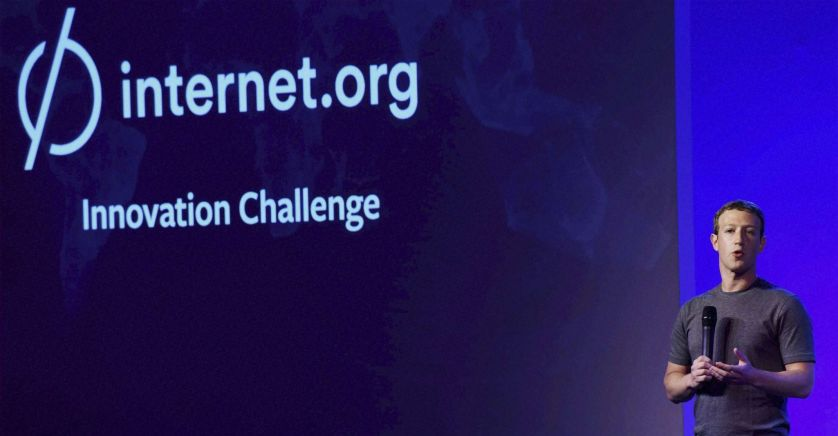
\includegraphics[scale=0.5]{orgConf}
    \caption{Zuckerberg stellt Internet.org auf der World Congress Conference vor\autocite{orgConf}.}
  \end{center}
\end{figure}
       
Mark Zuckerberg nennt drei Punkte, an denen man arbeiten muss, damit sich das Internet in den Entwicklungsländern ausbreiten kann
\parencite{HumanRight}:

\begin{itemize}
\item ``making internet access affordable by making it more efficient to deliver data."
\item ``using less data by improving the efficiency of the apps and experiences we use."
\item ``helping businesses drive internet access by developing a new model to get people online."  
\end{itemize}

Der erste Punkt zielt darauf ab, das Internet kostengünstiger/kostenlos anzubieten. 
Dies ist notwendig, damit auch Menschen mit einem geringen Einkommen es nutzen können.

Dazu ist es zunächst nötig den Datenverkehr effizienter gestalten, zum Beispiel durch leistungsfähigere Hardware.
Dies senkt Infrastrukturkosten für die Unternehmen, die diese bereitstellen.
Wenn dieser Profit an die Kunden weitergereicht wird, führt das zu einer Senkung der Internetkosten für den Einzelnen.

Zusätzlich könnte das dadurch entstehende überschüssige Kapital in den weiteren Ausbau des Netzwerkes investiert werden.

\medskip

Im zweite Punkt konzentriert sich Zuckerberg auf die Erhöhung der Leistungsfähigkeit von existierenden Dienstleistungen.
Es ist logisch: Weniger übertragene Daten entsprechen geringeren Kosten für den Nutzer.

\begin{quote}
``At Facebook, we’re investing heavily in opportunities to reduce our overall data use and help  other apps     
reduce their data use as well. Some of the areas we’re focused on are caching, data compression and simple efficiency optimizations.
- Mark Zuckerberg \textcite[8]{HumanRight}
\end{quote}

% cut
Die angesprochene Komprimierung kann man entweder durch die direkte Kompression von großen Apps realisieren oder indem man neue Dienstleistungen entwickelt, durch welche man seine Daten schicken und komprimieren lassen kann.

Facebook hat diese Mittel verwendet um den Datenverkehr effizienter zu gestalten.
Die Projekte Facebook Zero (Bereitstellung einer kostenlosen Internetverbindung, solange man sich auf Facebooks Webseiten befindet) und ``Facebook für jedes Handy" (eine Version von Facebook für feature Phones) wurden jeweils  2010 und 2011 eingeführt.
Facebook will die verwendete Technologie nun allgemein anwendbar machen, damit andere Dienstleistungen diese auch benutzen können.

\medskip

Mit dem letzten Punkt bekräftigt Zuckerberg den Glauben, die Ausbreitung des Internets sei die Aufgabe der Industrie , der Facebook mit Konzepten wie Internet.org zu Seite stehen möchte.

Dieses neue Konzept wurde dermaßen umgesetzt: Menschen in Entwicklungsländern sollen zuerst nur den kostenlosen Zugang zu grundlegenden Dienstleistungen wie Facebook haben.
Für diese Herangehensweise gab Facebook zwei Begründungen:
\medskip
Nicht jede Dienstleistung kann kostenlos bereitgestellt werden, da die dahinterstehenden Anbieter Profit erzielen müssen. 
Aber durch das kostenlose Bereitstellen grundlegender Anwendungen sei es möglich, den meisten Menschen Zugang zum Internet und der Industrie trotzdem indes den dabei größtmöglichen wirtschaftlichen Profit zu gewährleisten (wodurch diese wiederum mehr Zugang zum Internet bieten können).
Obwohl Zuckerberg sagt, dass er keine spezifische Gruppe von grundlegenden Internetdienstleistungen vorgibt, beschreibt er, welche Anwendungen er als grundlegend ansieht.

\begin{quote}
``many people who have never experienced the internet don’t know what a data plan is or why they’d want one. 
However, most people have heard of services like Facebook and messaging and they want access to them. If we can provide people 
with access to these services, then they’ll discover other content they want and begin to use 
and understand the broader internet." - \textcite[4]{HumanRight}
\end{quote}

Seiner Meinung nach sind es solche Dienstleistungen, die nicht viel Datenvolumen verbrauchen (hauptsächlich textbasierte und/oder einfach gehaltene Apps) und gleichzeitig auf andere Inhalte des Internets hin- oder verweisen.
Dienstleistungen, die unter diese Kriterien fallen, sind zum Beispiel Instant-Messaging-Dienste und soziale Netzwerke, Suchmaschinen und Enzyklopädien wie Wikipedia.(\cite[5]{HumanRight})
Dementsprechend ist Facebook Zuckerberg nach ein grundlegender Service, der eher als Andere kostenlos und überall zur Verfügung gestellt werden sollte.

\medskip

Facebooks Plan ist es diese Punkte unter dem Projekt Internet.org Industrie übergreifend zu bearbeiten.

% 1.2
\subsection{Ausgangssituation}

% 1.2.1
\subsubsection{Facebook}

Facebook erlebte ab 2011 ein starkes Wachstum an Nutzern in Indien, was 2012 mitunter durch die Beschränkung des Versendens von SMS auf maximal 200 pro Tag durch die TRAI (Telecom Regulatory Authority of India) unterstützt wurde, da Handybesitzer weiterhin unlimitiert kommunizieren wollten.
Dieses Kennenlernen und Nutzen von Facebook brachte den Teil der indische Gesellschaft, welcher bislang von der Globalisierung des Internets ausgeschlossen war, erstmals zur Bildung einer gemeinsamen, transnationalen Identität, was im Kontrast zur immer noch währenden Kastengesellschaft stand und steht.
Jene verwähren besonders Frauen den Zugriff auf soziale Medien und das Internet allgemein, die hohe Anzahl an Männern unter den Nutzern sei eine Gefahr für deren Keuschheit, doch selbst bei verheirateten Frauen wird häufig der Internetgebrauch durch zum Beispiel die Schwiegereltern überwacht.

\medskip

Besagte Überrepräsentation von jungen Männern zog unter anderem die Verbreitung der Misrepräsentation der eigenen Person online nach sich, was immer mehr zur Norm wurde.
Dies beinhaltet zumeist den Bildungsstand, den sozialen Hintergrund und Profilbilder. So wird ein Uniabbruch plötzlich zum bestandenen Bachelor, ein solcher zum sogennanten `Honours degree', eine höher gestellte Variante.

\medskip

Das Internet brachte jedoch auch Positives mit sich: da selbst gebildete Inder kaum mit der englischen Sprache vertraut waren, wurde das Erlernen und Lehren Anderer von der `Sprache des Internets" allgegenwärtig.
So bildeten sich Lerngruppen, welche sich in Internetcafe's trafen, um dort nicht nur Wissen, sondern auch den vergleichsweise teuren Datentarif zu teilen.

Neben diesen bleib auch die Internetgeschwindigkeit ein Problem, mit welcher die Inder eine durchschnittliche Seitenladezeit von 3,9 Sekunden hatten\autocite{mashable}.
Facebook versuchte auf dieses Problem mit der Messenger App einzugehen, in welcher nur Chats geladen werden, was aber nicht die endgültige Lösung darstellte.
Als eine weiterer Lösungsansatz gilt das Konzept für Internet.org.

% 1.2.2
\subsubsection{Internetverbreitung}

In Indien leben 2015 schon 350 Millionen Menschen welche das Internet aktiv nutzen\autocite{slideshareIndia}, wovon allein 159 Millionen per Mobilgerät unterwegs sind.
Obwohl Indien damit schon den 2. Platz der aktiven Internetnutzer weltweit genießt, haben lediglich 27\% der indischen Bevölkerung Zugang zum Internet\autocite{InternetCountry}.
\medskip 
Ein Computer ist in Indien ein Luxusgut, welches durch die rasante Entwicklung von mobilen Endgeräten für die Jugend schnell an Bedeutung verlor, während Handys mit mobilem Internet allgegenwärtig wurden.
Durch die explosionsartige Verbreitung der neuen Kommunikationsmöglichkeiten entstanden in kürzester Zeit große Gruppen im Internet, welche sich über neue Technologien, Wissenswertes und Ihre Interessen austauschten.
Dieser rapide Aufbau von individuellen Gruppen ist ein neues Phänomen, welches vor allem in Entwicklungsländern auftritt, in denen neue, und vergleichsweise preiswerte Technologien, den Zugang zum Internet ermöglichen \textcite{empowermentThroughFacebook}.
\medskip
Die durchschnittliche Bandbreite mobilen Internets war mit 2.8 Mb/s der durchschnittlichen Bandbreite eines Festanschlusses, von 2.3 Mb/s, überlegen \autocite{slideshareIndia}, wodurch das Interesse an einen Computer noch mehr abnahm.
Der Preis einer Prepaid Karte mit 1 GB Datenvolumen betrug damals ca. 3.55\% des durchschnittlichen Monatsgehalt\autocite{broadbandAgency}, und ist durch den hohen Preis nur für städtisch lebende Inder erschwinglich, da dort das Einkommen weitaus höher ist.
Obwohl gerade mal 31,2\% der indischen Bevölkerung in städtischen Gebieten lebt, machen sie 82\% der aktiven Internetnutzer aus\autocite{IndiaBevölkerung}.
Somit benutzten 2015 gerade mal 7.5 \%, auf dem Land lebende Inder, aktiv das Internet \autocite{slideshareIndia}.

Die fehlende weitreichende Abdeckung der Internetleitungen und der vergleichsweise hohe Datentarif sind schwerwiegende Probleme, welche Facebook inc. mit Internet.org lösen will.

% 1.2.3
\subsubsection{Netzneutralität} \label{netzneutralität}

Netzneutralität, oder `Net Neutrality' im Englischen, beschreibt ein Prinzip, nach welchem ein Internetanbieter allen Datenverkehr gleich behandelt, dass heißt ohne bestimmte Internetangebote langsamer oder teurer zu machen als andere \autocite{netzneutralität}.

\medskip

Indiens Vergangenheit ist im Bezug auf Netzneutralität noch sehr jung. So gab es vor Internet.org keine bestehende Verordnungen, und nur einige Vorfälle, welche eine Diskussion des Themas veranlassten.
Beide relevanten Debatten, ausgelöst vom lokalen Mobilfunkprovider Airtel, zielten darauf entgangene Gewinne des Konzerns ausgleichen zu lassen.
So wurde 2012 die Möglichkeit zur Besteuerung von Youtube, Google, Facebook, und Co. vorgeschlagen um für deren großen Teil am Datenverkehr zu kompensieren.
Auch 2014 ging es um eine ähnliche Problematik: so sollten VoIP (Voice over IP, Internettelefonie) Daten teurer sein als sonstige mobile Daten.
Beide Vorschläge führten zu keinem Ergebnis und wurden zum Teil stark von der Öffentlichkeit protestiert (Vgl. \textcite[253]{everydayLife} und \textcite{airtelVoip}).

% 1.2.4
\subsubsection{Aktivisten}

Die Seite, welche gegen Facebook argumentiert, sind die `Net Neutrality' Aktivisten, vereint unter dem Banner der `Save the Internet' Kampagne.
Zusammengesetzt aus Technologieinteressierten, primär den Mitarbeitern von Tech-Startups, die sich selbst als ``geeks and enthusiasts from various fields: technology, law, journalism, design, policy" \parencite{sti2015} beschreiben.

\medskip

Die Aktivisten können als eine `recursive public' verstanden werden. Welche von \textcite{twoBits} wie folgt definiert wird:

\medskip

\begin{quote}
A recursive public is a public that is constituted by a shared concern for maintaining the means of association through which they come together as a public.
Geeks find affinity with one another because they share an abiding moral imagination of the technical infrastructure, the Internet, that has allowed them to develop and maintain this affinity in the first place. - \cite[28]{twoBits}
\end{quote}

\medskip

Dies deckt sich mit dem Handeln der Aktivisten, welche sich über online Plattformen kennengelernt und unter dem gemeinsamen Ziel - das Internet wie sie es kennen (und lieben) zu verteidigen - vereinigt haben.

\medskip

Obwohl die Mitglieder von `Save the Internet' nur einen kleinen Teil der Bevölkerung repräsentieren, nämlich den der high-tech Arbeiter deren Anteil bei 2\% liegt (in einem Land in welchem 70\% der Menschen landwirtschaftlichen Tätigkeiten nachgehen), haben sie doch eine besondere Position inne. Denn sie spielen eine zentrale Rolle in der Vorstellung des neuen Indiens, welches in der globales Wirtschaft mitmischen kann (Vgl. \cite{thomas2012}).
Sie sind das Symbol der aufsteigenden Mittelschicht, welche durch Unternehmerschaft und harte Arbeit die indische Wirtschaft (7,7\% des 2,6 Billionen BIP 2017 \autocite{statistaIndiaGDP}\autocite{imfIndiaGDP}) und Indiens Position in der Welt voran treiben (8\% der Startups im Silicon Valley der 90er Jahre wurden von Indern angeführt \parencite{upadhya2004}).

\medskip

In Ihrer öffentlichen Präsentation ist die Initiative angelehnt an die `Net Neutrality' Bewegung der USA: von der Namensgebung und dem Logo über die verwendeten Hashtags in den sozialen Medien bis zu dem Vokabular mit welchem sie arbeiten (Vgl. \cite{prasad2017}).
Diese bewusst gewählten Assoziation mit dem erfolgreichen amerikanischen Modell, und auch die direkten Verweise auf westliche Popkultur, sollen die Kampagne für Ihre Zielgruppe ansprechender machen.

Die Zielgruppe setzt sich nicht aus den Menschen zusammen welchen Free Basics helfen möchte, sondern aus dem indische Mittelstand. Denn die Sprache mit der die Menschen angesprochen werden ist `Hinglish', ein Mix aus Hindi und Englisch, für deren Verständnis sowohl Englischkenntnisse - welche den Zugang zu neuen, qualifizierten Jobs ermöglichen und, ebenso wie eine Nähe zum Westen, die neue Mittelschicht Indiens prägen (Vgl. \cite{fernandes2006}) - als auch ein hohen Sprachniveau in Hindi voraussetzt.

\medskip

Ironischerweise, obwohl die Aktivisten gegen Facebook wettern, verbreiten sie Ihre Botschaft fast ausschließlich über soziale Medien, also auch zu großen Teilen über Facebook. Andere Kanäle um auf Ihre technopolitische (politische Meinungsbildung, getrieben durch Technologie) Kampagne aufmerksam zu machen sind u.a. (Vgl. \cite{prasad2017}):
\begin{itemize}
  \item YouTube: z.B. durch Erklärvideos einer angeheuerten komödischen Gruppe
  \item Ihr eigener Blog: in welchem die Probleme in einer seriöseren Form geschildert werden
  \item Twitter:
    \begin{itemize}
      \item zur direkten Interaktion untereinander und mit den Anhängern
      \item der Konfrontation mit Befürwortern von Internet.org
      \item um bei Tech-Firmen Gutheißungen für die Bewegung zu erbitten
    \end{itemize}
\end{itemize}

% 2
\section{Lebenszyklus der Initative}

Nachdem nun die Ausgangslage geschildert wurde, wird in diesem Teil der Verlauf des Projektes von der Einführung bis zum Verbot nach verfolgt.```

\subsection{Übersicht}

\definecolor{BGColor}{rgb}{1.0,1.0,1.0}
\begin{timeline}{2015}{2017}{250}{145}
  \MonthAndYearEvent{2}{2015}{Formeller Start}
  \MonthAndYearEvent{4}{2015}{Partielle Einführung}
  \MonthAndYearEvent{7}{2015}{Umbenennung zu Free Basics}
  \MonthAndYearEvent{11}{2015}{Vollständige Einführung}
  \MonthAndYearEvent{2}{2016}{Verbot}
\end{timeline}

Nur ein Jahr hat es vom offiziellen Start Anfang 2015, bis zum Verbot im Februar 2016 gedauert.

In der Zwischenzeit versuchte Facebook, nach initiellen Startschwierigkeiten, die Initiative durch ein Rebranding zu retten, was aber nicht reichte um die kritische Öffentlichkeit zu beeinflussen, deren Meinung bis zu den Entscheidungsträgern der zuständigen Behörde vordringen konnte.
Welche sich dann mit einem indirekten Verbot auf der Seite der Protestierenden positionierte.

% 2.2
\subsection{Formaler Start} \label{formal}

Nachdem \textcite{HumanRight} das Konzept vorstellte, wurde es nun durch die Partnerschaft mit dem Mobilfunkanbieter Reliance Realität.
Die Umsetzung sah folgendermaßen aus: Abonnenten von Reliance (solche im Besitz einer SIM Karte, nicht unbedigt eines laufenden Vertrages) haben die Möglichkeit über eine spezielle App auf den Seiten der Internet.org zu browsen.
Diese Implementation zieht aber einige große Probleme mit sich. So werden alle nicht-Reliance Abonenten ausgeschlossen was, da Reliance `nur' der viert Größte Anbieter mit 11\% Marktanteil\autocite{mobileSubscribers} ist, ein Großteil der Bevölkerung darstellt.

Auch lässt sich die Qualität (Geschwindigkeit) des Services, welche 4-12 mal langsamer ist, nicht mit der eines zahlenden Kunden vergleichen.
Die langsame Verbindung hat dabei mehrere Gründe. Zum einen wird die Bandbreite von Reliance gedrosselt um den zahlenden Abonnenten Vorrang zu verschaffen. Zu dem laufen alle Verbindungen durch einen Facebook Proxy Server in Europa, was dazu führt, dass die Route erheblich verlängert, erneut gedrosselt, und jegliche Verschlüsslung (TLS) umgangen wird(Vgl. \cite{walledGarden}).

\medskip

Zeitgleich kündigte Airtel, nachdem sie in der Vergangenheit schon mit der Idee experimentierten (beschrieben in Abschnitt \ref{netzneutralität}), ein ähnliches Konzept zu Internet.org an, bei welchem Firmen die Mobilfunkkosten für den kostenfreien Zugriff auf Ihre Services tragen würden.
Airtel's Ankündigung wurde mit einer Welle der Entrüstung aufgenommen, worauf hin Airtel auch schnell von der Idee abließ.
Dieser angesammelte Unmut wendete sich nun aber auch gegen Internet.org.

% 2.3
\subsection{Start in ausgewählten Regionen}

Im Anschluss an den formalen Start begann Facebook mit dem Aufsetzen der Netzinfrastruktur in den Regionen Tamil Nadu, Maharashtra, Andhra Pradesh, Gujarat, Kerala und Telangana.
Gleichzeitig fingen erneute Debatten um `Net-Neutrality' an Boden zu gewinnen.
Facebooks Dienst sei nicht konform mit dem Bestreben eines freien Internets, trotz der Bewerbung des Produkts als ``kostenloses Facebook" \parencite[3]{prasad2017}, später als ein ``step towards digital equality" (Ausführung in \ref{rebranding}).

\begin{figure}[h!]
  \begin{center}
    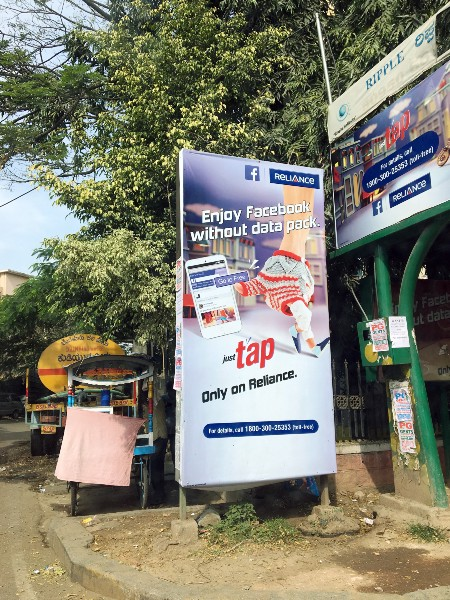
\includegraphics[scale=0.4]{wo-data-pack}
    \caption{Enjoy Facebook without data pack\autocite{woData}.}
  \end{center}
\end{figure}

In der ländlichen Bevölkerung gab es auch geteilte Meinungen hinsichtlich des Zugangs zum Internet, zumindest bei jenen, die sich selbst informiert haben oder informiert werden (von z.B. Nachrichtendiensten wie Digit.in) \parencite{digitYT}.
Hier kommt es jedoch zumeist zur Ignoranz des großen Ganzen, der Dienst wird als positiv entgegengenommen und genutzt, Aktionen wie die wortwörtlich vorgeschriebene Unterschreibung zugunsten von Facebook in der Debatte um Netzneutralität\autocite{ndtvYT} werden ohne weiteres Hinterfragen und potenziell aufgrund von Unwissen unterstützt.
Einzig ein initielles Interesse an einem kostenlosen Dienst im allgemeinen Sinne ist ein gemeines Ziel.

\medskip

Anzumerken bei alledem ist, dass der Großteil der Bevölkerungsgruppe, die in Facebooks Werbekampanien als Zielgruppe des Dienstes beschrieben werden, entweder keinen, oder nur einen geringfügigen Nutzen genießt.
Jene, die sich den Besitz eines digitalen Endgeräts (id est Smartphones, etc.) leisten können, sind aufgrund der geringen Preise auch in der Lage, eine stabilere und schnellere Internetverbindung als Facebooks Dienst sie anbietet, zu erwerben.
Der Rest, also Personen, die (zu Teilen weit) unterhalb der Armutsgrenze leben, haben weder Wege, Internet.org zu nutzen, noch einen Grund dafür \parencite[257]{everydayLife}.

\medskip

So ist die Nutzung des Dienstes selbst fern vom beinahe utopischen Beispiel von Facebooks Seite des Landwirts Ganesh, welcher mithilfe von Internet.org seinen Ertrag verdoppelte, indem er Informationen über das Wetter und aktuelle Warenpreise nutzt, ein Beispiel für die Angabe, dass für alle 10 Teilnehmer an Internet.org eine Person aus der Armut gehoben wird \parencite[4]{prasad2017}.
In der Realität besteht die Nutzerbasis wie besagt aus männlichen Jugendlichen und jungen Erwachsenen.
Hier wurde Facebook zu einem Bestandteil des Lebens, der sich fast virusartig durch persönliche Weiterempfehlung verbreitete.
Dies geht über zu spezialisierten Kursen von neuen oder schon vorher `Tech-Affinen', die Teilnehmern Grundlegendes von der Inbetriebnahme von Smartphones bis zum Kommentieren bei Facebook beibringen \parencite{empowermentThroughFacebook}.

\medskip

Dies allein ist natürlich keine schlechte Sache; besagte Menschen gehören zu einer Generation von Gelehrten, jedoch aufgrund der hohen Mensch- zu Arbeitsplatzratio zumeist arbeitslosen, zwanzig- bis dreißigjährigen Indern, die sich von der Welt abgehängt fühlen.
Eine Lehrfunktion bietet eben solchen neben Arbeit auch einen Daseinszweck.

\medskip

Besagte Kurse brachten einen weiteren positiven Effekt mit sich, die Verbreitung des Englischen durch Selbstbeibringung in Gebieten, in denen vorher weder Englisch noch Hindi gesprochen wurde \parencite{empowermentThroughFacebook}. Die Tatsache, dass der Großteil der Analphabeten vor Allem unter der genannten Gruppe, welche unter der Armutsgrenze lebt, zu finden sind, bleibt hierbei leider bestehen.

\medskip

Ferner stehen positiven Aspekten weitere bereits etablierte soziale Normen im Wege; Informationsverbreitung geschieht im ländlichen Indien immer noch zu großen Teilen über Mundpropaganda \parencite[259]{everydayLife}, Mädchen wird Zugriff auf Medien zugunsten des (erstgeborenen) Jungen verwährt \parencite{empowermentThroughFacebook} und soziale Gruppierungen werden vom Realen ins Virtuelle übernommen.

\medskip

% cut
All dies hätte sich nicht durch eine ausschließlich kostenpflichtige Variante des Internets geändert.
Allein die Zahlen der nationalen Internetverbreitungsrate (2016 25\% $\to$ 2019 50\%) sprechen für eine graduelle Veränderung gen Akzeptanz bezüglich des Internets.

% 2.4
\subsection{Rebranding als Free Basics} \label{rebranding}

\begin{figure}[h!]
  \begin{center}
    
\includegraphics[scale=0.6]{intro}
    \caption{Introducing: free basics by facebook\autocite{introFB}.}
  \end{center}
\end{figure}

Drei Monate nach dem Start von Internet.org begann die indische Regierung unter Premierminister Narendra Modi die `Digital India campaign' mit Zielen wie erweiterter Breitbandkonnektivität, Universalzugang zu Mobilnetzen und einem Programm für öffentlichen Internetzugang \parencite{digitalPillars}.
Hierfür trat die Regierung mit Firmen des Silicon Valley in Kooperation, unter anderem Facebook (Bereitstellung von Wifi Hotspots in ländlichen Gebieten) \parencite[254]{everydayLife},
wobei Modi und Zuckerberg ein öffentliches Image der engeren Zusammenarbeit aufbauten.

\medskip

Dies führte selbstverständlich zu weiteren Unruhen unter den wachsenden Protesten gegen Internet.org, welche sich von nur wenigen Teilnehmern Anfang April, zu global verteilten Kommentaren zuwider Facebook eineinhalb Monate später ausweiteten \autocite{BBC3}.
Während diese primär online abliefen, fingen Menschen an auf die Straße zu gehen.

\medskip

Zuckerbergs reaktive Äußerung ``universal connectivity and net neutrality can and must co-exist", wobei der Dienst erstmalig als ``basic free services" bezeichnet wurde, ließen die Stimmen (der `Safe The Internet coalition') lediglich lauter erklingen.
Wenige Wochen später unterschrieben 67 sog. `digital rights' Aktivistengruppen (u.A. `i Freedom Uganda', `Usarios Digitales' aus Equador und `ICT Watch' aus Indosnesien) einen an Facebook gerichteten Brief über Bedenken am Projekt.

\medskip

Nachdem weitere Unternehmen aufgrund der Proteste austraten, gab Facebook den größten Stimmen nach. Unter dem neuen Namen `Free Basics' lockerte Facebook die Vorgaben für Webseiten Betreiber und erlaubte die Verwendung von HTTPS, was gemeinsam zu einer Erweiterung des Angebots um 60 neue Seiten führte.

% 2.5
\subsection{Nationaler Start} \label{national}

Der nationale Start von Internet.org's Free Basics App begann im November 2015. Nutzer hatten nun Zugriff auf Wikipedia, Bing, BBC News, soweiso einige lokale Nachrichtendienste.
Google Austritt aus der Free Basics führte zu mehr Skepsis gegenüber Facebooks Plattform.
Hinzu kommt, dass sich Google CEO Sundar Pichai positiv in der Debatte um Netzneutralität aussprach \parencite{easeOfBusiness}.

Ein größeres Problem bestand auch darin, wie Facebooks Projekt in Indien wahrgenommen wurde im Kontrast zu ihrer eigenen Werbekampagne.
Free Basics, sofern überhaupt von der Bevölkerung wahrgenommen, wird von vielen Indern als Werbung für Facebook und Reliance angesehen.
Dies steht kritisch in Relation zu ihren eigenen Behauptungen, man versuche der armen Landbevölkerung gleichwertigen Zugriff auf Informationen durch das Medium Internet zu gewähren \parencite[4]{everydayLife}.
Aufgrund der geringen Anzahl an verfügbaren Webseiten und der schlechten Geschwindigkeiten (Vgl. Abschnitt \ref{formal}) stellt das Angebot für die Nutzer keine wirkliche Alternative dar, weshalb sich die Nutzer vom Projekt abwenden\autocite{nyt1}.
	
% 2.6
\subsection{Verbot durch Regulatoren}

Noch in Mitten des Austausches über das Pro und Contra der Netzneutralität veranlasste TRAI im Dezember 2015 eine Anordnung an Reliance Communications Facebook's Free Basics vorläufig zu sperren\autocite{governanceAsIdeology}.
Facebooks `Save Free Basics' Kampagne im Januar 2016 sorgte dann nur für weiteres Misstrauen.

Im Februar 2016 verabschiedete TRAI daraufhin die \textcite{regulationBan}.
In dieser Verordnung legte die Behörde fest, dass von Telekommunikationsanbietern geschlossene Verträge und Tarife mit Kunden nicht zwischen Inhalten bzw. Websites differenzieren dürfen.
Sie beruft sich dabei auf die Prinzipien der Netzneutralität (Vgl. Abschnitt \ref{netzneutralität}).

Basierend darauf wurde entschieden, dass Free Basics, welches freien Zugang zu kooperierenden Diensten ermöglicht, den
Verordnungen widerspricht und folgegemäß ab dem 8. Februar 2016 offiziell in Indien verboten sei.

\break
\section{Fazit}

Aus unseren zusammengetragenen Informationen lässt sich erschließen, dass das Projekt Internet.org/Free Basics in Indien in kurzer Zeit (Start Februar 2015; Verbot Februar 2016) unter anderem durch öffentliche Kritik gescheitert ist.
Der von Facebook angezielte Markt war durch ein ähnliches und bereits unter Feuer geratenes Projekt nur Monate vorher verstimmt worden, fehlerhaftes Management, insbesondere die Stimme an Presse und Bevölkerung nahm nur selten an der Diskussion um tatsächlich besprochene Kitikpunke teil, wobei selbst dann nur das eigene Projekt verteidigt wurde.
Als im September endlich nachgelassen wurde, war es bereits zu spät; die Bevölkerung stimmte der Opposition zu, was final in der Entscheidung des TRAI resultierte.

\medskip

Die anbeginns formulierte Frage, ob Zuckerbergs Versprechen, Teile der untersten Schicht durch Zugriff auf das Internet aus der Armut zu heben, nachgekommen wurde, lässt sich klar verneinen.

Das Projekt kann weder als Erfolg für seine Zielgruppe noch für Facebook gewertet werden. So konnten die Probleme der Zielgruppe, wie mangelndem Zugriff auf internetfähige Geräte, unzureichender Verfügbarkeit, einem schwachen Service und der Missachtung der Rolle von Frauen in der Gesellschaft, nicht durch kostenlosen Zugang zum Internet behoben werden. Trotz hoher Investitionen könnte Facebook die Öffentlichkeit nicht für sich gewinnen und wurden durch die, an dem Erhalt eines offenen und fairen Internet interessierten, `Technologists' der `Save the Internet' Kampagne ausgeboten.

\break
\appendix
\section{\\Meinungen zum Projekt}

Man kann Free Basics verschieden beurteilen. Meiner Meinung nach [Jonathan Neidel] hat Facebook viel versprochen, das ganze dann als eine Marketing Kampagne für Ihre Platform genutzt, aber am Ende nichts geliefert. Durch Reliance als Partner war die Anzahl der von der Intiative betroffenen Menschen sehr gering (im Vergleich zu ihrem `Weltretter' Marketing) und auch die schlechte Servicequalität sorgt für eine Zwei-Klassen Gesellschaft. Wenn man dann noch die Statistik in Betracht zieht, dass 50\% der Nutzer nach dem ersten Monat einen Vertrag abschließen \parencite{everydayLife}, dann ist Free Basics nicht mehr als ein glorifiziertes (Facebook) Probeabo und nicht die versprochene Langzeitlösung für die ärmste Bevölkerungsschicht.

\medskip

Aus meiner Sicht [Sarah Susanne Fischer] hätte Facebook von Anfang an anders handeln müssen, wenn sie wirklich nur philanthropische Absichten gehabt hätten. Bereits bei der Planung des Projektes war es für Facebook klar, dass sie keine bzw. eine komplementäre Kommunikation mit der Bevölkerung Indiens führen werden. Zuckerberg war der Meinung, dass die Menschen aus den Entwicklungsländern das Internet, wie wir es kennen, nicht verstehen würden. Dadurch hat er diese Menschen auf eine niedrigere Stufe gestellt und es als angebracht betrachtet diese zu bevormunden. 
Dies bestärkt den Eindruck dass Facebooks Absichten nicht so human waren, wie sie den Anschein erwecken wollten.

\medskip

Meiner Meinung nach [Oliver Hein] ist die Idee, Internet in Entwicklungsländern erschwinglich für jede Bevölkerungsschicht verfügbar zu machen ein ehrhafter Ansatz, aber die Umsetzung von Facebook war schwach. Die Eingrenzung der Verfügbarkeit von Internetseiten spricht gegen die freie Meinungsbildung und die Kommunikation zwischen Facebook und der Bevölkerungsschicht, die es betrifft mangelhaft bis gar nicht vorhanden.

\medskip

Meiner Meinung nach [Tom M. P.] stand primär die Behandlung der öffentlichen Kritik dem Erfolg im Wege.
Während zu Beginn tatsächliche Nutzer und selbst der Premierminister vom Konzept überzeugt waren, wurden solche Stimmen schnell übertönt, was dazu führte, dass als endlich Änderungen vorgenommen wurden.
Meiner Einschätzung nach selbst extremere Maßnahmen (wie zum Beispiel die Unterstützung direkter Konkurrenz, eine Free Basics-kompatible Variante ihres Dienstes zu erstellen) als tatsächlich Eingeführte geholfen hätten.
Vielleicht wäre ein partieller Erfolg möglich gewesen, wenn Facebook früher (bereits Anfang April) in Aktion und Konversation mit der Gegenseite getreten wäre.
Weiterhin bin ich trotzdem gespannt, welche Strategien in der Zukunft noch versucht werden, um Indiens Markt an Konsumenten zu erfassen.

\break
\printbibliography

\end{document}
